\begin{pastexam}[label={px:ntu-109-comm-dsa-50}]{臺大電信所 109 學年度（B）第 50 題}
（複選；每題 2 分，每答錯一個選項倒扣 0.4 分）

Consider the Fibonacci heap in Fig.3
\begin{enumerate}[label=(\Alph*),nosep]
\item In Fig.3, after decreasing key 89 to 40, there will be 3 marked nodes in total.
\item In Fig.3, after decreasing key 59 to 40, there will be 5 marked nodes in total.
\item In Fig.3, after decreasing key 15 to 10, there will be 2 trees in total.
\item In Fig.3, after delete-min, there will be two trees.
\item In Fig.3, after inserting key 68, there will be one tree.
\end{enumerate}

\begin{center}
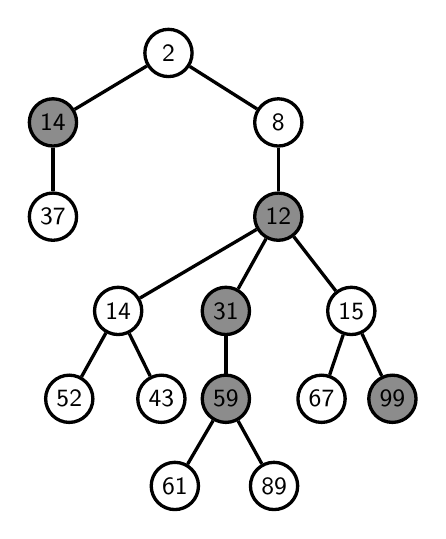
\begin{tikzpicture}[scale=0.9, v/.style={circle,draw,minimum size=6mm,inner sep=0pt,font=\small\sffamily,very thick}]
\node[v] (2) at (3.23,-0.87) {2};
\node[v,fill=black!45] (14m) at (1.60,-1.85) {14};
\node[v] (8) at (4.78,-1.85) {8};
\node[v] (37) at (1.60,-3.18) {37};
\node[v,fill=black!45] (12) at (4.78,-3.18) {12};
\node[v] (14) at (2.52,-4.51) {14};
\node[v,fill=black!45] (31) at (4.04,-4.51) {31};
\node[v] (15) at (5.81,-4.51) {15};
\node[v] (52) at (1.83,-5.75) {52};
\node[v] (43) at (3.13,-5.75) {43};
\node[v,fill=black!45] (59) at (4.04,-5.75) {59};
\node[v] (67) at (5.39,-5.75) {67};
\node[v,fill=black!45] (99) at (6.39,-5.75) {99};
\node[v] (61) at (3.32,-6.98) {61};
\node[v] (89) at (4.72,-6.98) {89};
\draw[very thick] (2) -- (14m); \draw[very thick] (2) -- (8);
\draw[very thick] (14m) -- (37); \draw[very thick] (8) -- (12);
\draw[very thick] (12) -- (14); \draw[very thick] (12) -- (31); \draw[very thick] (12) -- (15);
\draw[very thick] (14) -- (52); \draw[very thick] (14) -- (43);
\draw[very thick] (31) -- (59);
\draw[very thick] (15) -- (67); \draw[very thick] (15) -- (99);
\draw[very thick] (59) -- (61); \draw[very thick] (59) -- (89);
\end{tikzpicture}

Fig.3 Fibonacci heap
\end{center}
\end{pastexam}

\begin{pastsoln}
答案：(A)(B)。

圖中灰底的是有標記（marked）的節點：根 $2$ 左邊的 $14$、$12$、$31$、$59$、$99$，共 $5$ 個。 整個堆積
只有一棵樹，根是 $2$。 以下照資結書第~8.6~節的操作；每個選項都從原圖開始。

\textbf{(A) 89 減成 40：對。} $40 < 59$（父節點），把 $40$ 剪下放進根串列。 父節點 $59$ 有標記，
連鎖剪下：$59$ 剪下、去掉標記；它的父節點 $31$ 也有標記，剪下、去掉標記；再往上 $12$ 有標記，
剪下、去掉標記；再往上 $8$ 沒有標記，而且不是根，給它加上標記，停止。 原本的標記
$\{14, 12, 31, 59, 99\}$ 去掉 $12, 31, 59$，加上 $8$，剩 $\{14, 99, 8\}$，共 $3$ 個。 （根串列變成
$2, 40, 59, 31, 12$ 五棵樹。）

\textbf{(B) 59 減成 40：對。} $59$ 的父節點是 $31$，$40 \ge 31$，堆積性質沒有被破壞，不用剪，只改
鍵值。 標記不變，仍是 $5$ 個。

\textbf{(C) 15 減成 10：錯。} $10 < 12$（父節點），剪下 $10$ 放進根串列。 $12$ 有標記，連鎖剪下 $12$
並去掉標記；$8$ 沒有標記，加上標記，停止。 根串列有 $2$、$10$、$12$ 三棵樹，不是 $2$ 棵。

\textbf{(D) delete-min：錯。} 拿掉最小的根 $2$，它的兩個子節點 $14$（子樹 $14 \to 37$）和 $8$（子樹
$8 \to 12 \to \cdots$）放進根串列，再整理：兩棵的根都只有 $1$ 個子節點，階數都是 $1$，要連結成一棵。
$8 < 14$，$14$ 那棵掛到 $8$ 底下，$8$ 的階數變成 $2$。 最後只剩\textbf{一棵}樹，最小值是 $8$。

\textbf{(E) 插入 68：錯。} 插入只把新節點放進根串列，不做連結，所以有 $2$ 和 $68$ 兩棵樹。
\end{pastsoln}
